%%%%%%%%%%%%%%%%%%%%%%%%%%%%%%%%%%%%%%%%%%%%%%%%%%%%%%%%%%%
% --------------------------------------------------------
% Rho
% LaTeX Template
% Version 2.1.1 (01/09/2024)
%
% Authors: 
% Guillermo Jimenez (memo.notess1@gmail.com)
% Eduardo Gracidas (eduardo.gracidas29@gmail.com)
% 
% License:
% Creative Commons CC BY 4.0
% --------------------------------------------------------
%%%%%%%%%%%%%%%%%%%%%%%%%%%%%%%%%%%%%%%%%%%%%%%%%%%%%%%%%%%

\documentclass[9pt,a4paper,twoside]{rho-class/rho}
\usepackage[english]{babel}

%% Spanish babel recomendation
% \usepackage[spanish,es-nodecimaldot,es-noindentfirst]{babel}

\setbool{rho-abstract}{true} % Set false to hide the abstract
\setbool{corres-info}{true} % Set false to hide the corresponding author section

%----------------------------------------------------------
% TITLE
%----------------------------------------------------------

%\journalname{Molecular Ecology}
\title{Genome-Wide Analysis Reveals Altitude-Associated Divergence in a Color-Polymorphic Insect}
%----------------------------------------------------------
% AUTHORS AND AFFILIATIONS
%----------------------------------------------------------

\author{}

%----------------------------------------------------------

\affil{}

%----------------------------------------------------------
% DATES
%----------------------------------------------------------

\dates{This manuscript was compiled on May 27, 2025}

%----------------------------------------------------------
% FOOTER INFORMATION
%----------------------------------------------------------

\leadauthor{}
\smalltitle{Altitude-Driven Adaptive Divergence}

%----------------------------------------------------------
% ARTICLE INFORMATION
%----------------------------------------------------------

\corres{}
\email{}

%----------------------------------------------------------
% ABSTRACT
%----------------------------------------------------------

\begin{abstract}
    Environmental gradients are key drivers of genetic and phenotypic variation, yet the genomic basis of adaptation across steep altitudinal clines remains understudied. We examined a montane insect, \textit{Isophya rizeensis}, exhibiting discrete color polymorphism along a 450–2,300 m elevation gradient in the Fırtına Valley of Türkiye. Using genome-wide RAD sequencing of 71 individuals, we identified over 92,000 SNPs, including 1,113 putatively adaptive loci. Despite low overall genetic differentiation, adaptive loci showed stronger divergence and 101 SNPs were significantly associated with altitude, displaying reciprocal allele frequency shifts. Discriminant analysis revealed three major-effect loci distinguishing dark and pale color morphs, all linked to elevation. These findings are consistent with spatially varying selection maintaining adaptive genetic variation and phenotypic polymorphism despite gene flow. Our results provide insights into the genetic architecture of local adaptation and contribute to understanding how environmental heterogeneity shapes biodiversity in montane ecosystems.
\end{abstract}

%----------------------------------------------------------

\keywords{Clinal variation, Local adaptation, Genotype–environment association, RAD sequencing, Adaptive divergence, Non-model insect}

%----------------------------------------------------------

\begin{document}
	
    \maketitle
    \thispagestyle{firststyle}
    % \tableofcontents
    \linenumbers

%----------------------------------------------------------

\section{Introduction}

    Understanding how environmental gradients shape genetic and phenotypic variation is a central question in evolutionary ecology. Altitudinal and latitudinal gradients, in particular, serve as powerful natural laboratories for examining the interplay between gene flow, selection, and drift across spatially variable environments (\cite{Wogan2018}; \cite{Kelly2019}). These gradients impose structured ecological variation—such as shifts in temperature, humidity, and oxygen availability—that can drive local adaptation by favoring different alleles or traits at different elevations (\cite{Muir2014}). By investigating how genomic and phenotypic diversity align with these gradients, researchers can uncover the evolutionary mechanisms that underlie population differentiation and adaptation (\cite{Merilä2014}; \cite{Waldvogel2020}).

    Altitudinal gradients are especially informative because they generate sharp environmental transitions over short geographic distances (\cite{Chown2003}; \cite{Flatt2016}). \textcolor{PineGreen}{These transitions can reduce gene flow and strengthen divergent selection. The resulting spatial structuring may amplify the effects of isolation by distance (IBD), a process where genetic similarity decreases with geographic distance (\cite{Orsini2013}). At the same time, strong selective pressures including temperature variation, hypoxia, and shifts in vegetation structure can drive genetic differentiation through local adaptation (\cite{Sexton2014}; \cite{Stankowski2017}; \cite{Bradburd2019}). Combined with tools like genotype–environment association (GEA) analyses, altitudinal clines have become a valuable framework for identifying genetic loci under spatially varying selection (\cite{Hancock2011}; \cite{Slatyer2014}; \cite{Pluess2016}). In many systems, clinal variation in traits or allele frequencies provides insight into how selection acts across heterogeneous landscapes (\cite{Mayekar2022}; \cite{Tyrmi2020}; \cite{Soliani2020})}.

    One well-documented axis of altitudinal divergence is color polymorphism, especially in invertebrates. Color traits in insects are often involved in thermoregulation, camouflage, and ecological specialization, influencing both survival and fitness (\cite{Forsman2008}; \cite{Zeuss2014}; \cite{Kozlov2022}). Thermal melanism—the tendency for darker individuals to occur in colder, higher elevations—is a widely reported pattern, attributed to the thermal benefits of increased solar absorption (\cite{Clusella-Trullas2020}). Nevertheless, many ectothermic species deviate from this pattern, indicating that additional ecological drivers, such as habitat complexity and predation, also play important roles in the evolution of color traits (\cite{Karlsson2008}; \cite{Goodman2021}).

    Beyond thermoregulation, color polymorphism can expand niche breadth by \textcolor{PineGreen}{enabling different color morphs to perform optimally under distinct microclimatic or habitat conditions, thereby allowing populations to occupy a wider range of environmental conditions}. This promotes broader distribution, ecological resilience, and potentially reduces extinction risk under environmental change (\cite{Forsman2008}; \cite{Wennersten2009}; \cite{Kozlov2022}). Understanding the genetic basis of such variation is essential for linking phenotypic divergence to evolutionary processes and identifying the drivers of population persistence and speciation (\cite{Forsman2016}; \cite{McLean2014}).

    In this context, the montane bush cricket \textit{Isophya rizeensis} (Orthoptera: Tettigoniidae: Phaneropterinae: Barbitistini) provides an exceptional system for studying altitudinal adaptation (\cite{SEVGILI2003}). \textcolor{PineGreen}{The species is narrowly endemic to the Fırtına Valley and neighbouring valleys of the Pontic Mountains, where its distribution is highly fragmented and mostly restricted to isolated subalpine patches above approximately 1,600 m (Figure 1). Notably, the Fırtına Valley is the only known location where \textit{I. rizeensis} occurs continuously from lowland habitats (~300 m) up to 2,400 m. This provides a uniquely complete low-to-high elevation transect, making it an ideal system for investigating clinal patterns of genomic and phenotypic divergence (Figure 1)}.
    
    \textcolor{PineGreen}{Along the elevation gradient within the Fırtına Valley, vegetation changes markedly: densely shaded Colchic broadleaf and boxwood forests dominate the lower valley (<900 m), cooler mixed beech–spruce–fir stands occur at mid-elevations, and open, sparsely vegetated subalpine meadows are found above ~1,800 m, where solar exposure is high and thermal conditions are more extreme (\cite{Karacaoglu2014}). Within this environmental mosaic, males exhibit pronounced dorsal colour polymorphism. Dark individuals are found at lower elevations (350–1000 m), while pale morphs occur at higher altitudes (1100–2300 m). Populations along this gradient are typically monomorphic for a single colour, with a discrete transition between dark and pale forms occurring near ~1,100 m (\cite{SaglamCaglar2005}; \cite{SaglamCaglar2007Isophya}; \cite{Çağlar2014})}. This distribution contrasts with the expectations of classical thermal melanism, which predicts darker phenotypes at cooler, higher elevations (\cite{CLUSELLATRULLAS2007}). \textcolor{PineGreen}{Females also vary in coloration, but only subtly and without the discrete black–green divergence observed in males (\cite{SEVGILI2003}; \cite{SaglamCaglar2005})}.
    
    Physiological data suggest that darker males warm more quickly and reach higher body temperatures than paler ones, which could be maladaptive in subalpine habitats where surface temperatures regularly exceed 40°C due to intense solar radiation (\cite{Kuyucu2016}). In such environments, paler coloration may reduce overheating risk, offering a selective advantage in sparsely vegetated, high-altitude zones. Despite these observations, the genetic architecture underlying this color polymorphism and its relationship with elevation and population differentiation are not yet understood. Furthermore, it remains to be determined whether phenotypic divergence is maintained by selection or results from neutral processes such as drift and limited gene flow.
    
    \textcolor{PineGreen}{Here, we investigate the genomic basis and maintenance of colour polymorphism along an altitudinal gradient by integrating genome-wide RAD sequencing with population genetic and genotype–phenotype association analyses. Our study focuses on male phenotypes, in which colour morphs are discrete, spatially structured, and ecologically well characterized (\cite{Çağlar2014}).} Specifically, we aim to:

    \begin{enumerate}
    \item Characterize population structure and connectivity along an altitudinal gradient.
    \item \textcolor{PineGreen}{Disentangle between neutral and adaptive genetic differentiation}.
    \item Identify loci associated with altitude and color polymorphism, clarifying whether these patterns arise from a common genetic basis.
    \end{enumerate}

    By coupling genomic data with environmental and phenotypic gradients, our study sheds light on the mechanisms driving local adaptation and the maintenance of intraspecific diversity in heterogeneous montane ecosystems. We show that a small subset of adaptive loci can remain highly differentiated despite extensive gene flow across a narrow altitudinal gradient, providing insight into how spatially varying selection may contribute to the maintenance of functional polymorphism. Our reference-free analytical framework is broadly applicable to non-model taxa, and our findings contribute to ongoing debates about the genomic architecture of local adaptation. More broadly, this work offers empirical grounding for forecasting the evolutionary resilience of montane biodiversity under accelerating environmental change.

\section{Materials and Methods}

    \subsection{Sample Collection and Sequencing}

        Male specimens used in this study were collected between June and August 2006 from 11 locations along an altitudinal gradient ranging from 450 to 2,300 meters above sea level in the Fırtına Valley (Figure 1) via sweep netting and categorized according to color as described in \cite{Çağlar2014}. DNA was extracted from the hind femora of individuals using the \textsc{E.Z.N.A.}® Insect DNA Kit (Omega Bio-Tek), following the manufacturer’s protocol. Genome-wide data were generated via Restriction site–Associated DNA sequencing (i.e., RAD sequencing). Paired-end RAD libraries were constructed using the \textit{PstI} restriction enzyme, following the protocol detailed in \cite{Ali2016} \textcolor{PineGreen}{(see \textbf{Supporting Information: RAD Library Preparation} for details)}. Sequencing was conducted at an average depth of 10× on an Illumina HiSeq4000 at the UC Davis Genome Center. In total, we generated RAD sequencing data from 75 \textit{I. rizeensis} individuals along the Fırtına Valley, averaging 5–7 individuals per location/altitude.
    
    \subsection{Alignment and filtering}

        Due to the absence of a reference genome for \textit{I. rizeensis} or \textcolor{PineGreen}{any} closely related species, we generated a de novo RAD sequence reference library following the custom procedure given in \cite{SağlamMolEcol2016} \textcolor{PineGreen}{(see \textbf{Supporting Information: De-novo RAD locus discovery and extension} for details)}. Raw reads from each individual were aligned to the reference set of RAD-contigs using the \textsc{bwa-mem} algorithm (\cite{Li2010}; \cite{Li2013}). The resulting \textsc{sam} files were converted to coordinate-sorted \textsc{bam} files using \textsc{samtools} (\cite{Danecek2021}), and duplicate reads were marked with \textsc{Picard tools} (http://broadinstitute.github.io/picard). Paralog regions (i.e. RAD-contigs) were identified using \textsc{ngsParalog} (https://github.com/tplinderoth/ngsParalog) and removed from subsequent analysis.

    \subsection{SNP discovery and genotyping}

        Polymorphic sites were identified using \textsc{angsd}  (\cite{Korneliussen2014}) by calculating genotype likelihoods (\texttt{-GL $1$}), major and minor alleles (\texttt{-doMajorMinor $1$}), minor allele frequencies (\texttt{-doMaf $1$}), and generating \textsc{BCF/VCF} files (\texttt{-doBcf $1$}). Polymorphic sites were filtered to include only those with a minor allele frequency (MAF) of $0.05$ or higher (\texttt{-minMaf 0.05}). Additional filtering parameters included a minimum base quality score of $20$ (\texttt{-minQ $20$}), a minimum mapping quality of $10$ (\texttt{-minMapQ $10$}), and a posterior genotype probability threshold of $0.85$ (\texttt{-postCutoff $0.85$}). Only properly paired reads ( \texttt{-only\_proper\_pairs $1$}) were considered, and sites were retained only if the probability of them being polymorphic was statistically significant (\textit{P} < $10^{-12}$). Finally we filtered out any site that had an average per individual read depth under $6X$ and was not present in at least $50\%$ of individuals in each population.

    \subsection{Population Genetic Structure}

        Population genetic structure was assessed using Principal Component Analysis (PCA). First, a genetic covariance matrix was calculated between individuals in \textsc{PCAngsd} (\cite{Meisner2018}) based on genotype likelihoods. The covariance matrix was then subjected to eigenvalue decomposition in R (\cite{R2024}, version 4.2.0) to extract the principal component axes summarizing genetic variation and the first two principal components (PCs) were visualized in R.
       
        Admixture analyses were conducted with \textsc{NgsAdmix} (\cite{Skotte2013}) to estimate individual ancestry proportions based on genotype likelihoods. Analyses were performed for K values ranging from 2-5, with 10 independent runs for each K value to account for stochastic variation and avoid convergence to local optima. \textcolor{PineGreen}{We restricted admixture inference to a maximum K of 5 to minimize the risk of overfitting and spurious clustering, which can occur when population structure is weak or continuous (\cite{Lawson2018})}.The most likely number of clusters was identified using the $\Delta{K}$ method of \cite{Evanno2005}, which calculates the rate of change in log-likelihood values across successive K values and admixture proportions for each K value were visualized in R.

    \subsection{Genetic Differentiation and Isolation By Distance (IBD)}
    
        \textcolor{PineGreen}{Genetic differentiation among sampling sites along the altitudinal gradient was assessed using pairwise $F_{ST}$. Genome-wide $F_{ST}$ values were estimated in \textsc{ANGSD} using a likelihood-based framework that integrates genotype likelihoods rather than hard genotype calls. For each population pair, site allele frequency likelihoods were computed for all variable sites, and a joint 2-dimensional site frequency spectrum (2D-SFS) was estimated with the \texttt{realSFS} module. Global weighted F$_{ST}$ values, representing genome-wide weighted averages of site differentiation, were then computed with \texttt{realSFS} using the \texttt{-whichFst 1} estimator (\cite{Nielsen2012}) which provides more accurate estimates when working with moderate sample sizes (5–7 diploid individuals; i.e., 10–14 independent chromosome copies) (\cite{Willing2012}). Importantly, folded site frequency spectra inferred for each locality were well formed and highly similar across elevations (Supplementary Figure S1), indicating that allele-frequency estimates and downstream differentiation metrics were not driven by elevation-dependent allelic dropout or sampling bias.}
        
        To evaluate patterns of isolation by distance (IBD), a Mantel test was performed to assess the correlation between geographic and genetic distances. A Euclidean distance matrix between populations was generated using the \textsc{Geographic Distance Matrix Generator} v1.2.3 (\Cite{Ersts2024}) and served as the predictor variable, while the linearized pairwise $F_{ST}$ matrix [$F_{ST}$/(1 - $F_{ST}$)] was used as the response variable. IBD patterns were analyzed through Pearson and Spearman correlation Mantel tests with 999 permutations, implemented in R using the \texttt{vegan package} (\cite{Oksanen2001}; \cite{Mantel1967}).
 
    \subsection{Comparing Neutral and Adaptive Genetic Variation}

        \textcolor{PineGreen}{To identify putatively adaptive loci, we used the \texttt{Pcadapt} implementation in \texttt{PCAngsd} (\cite{Meisner2018}), which detects SNPs whose allele-frequency variation is significantly associated with major axes of genetic structure inferred from principal components (\cite{Luu2017}). Unlike $F_{ST}$-based outlier approaches that require predefined population groupings and identify loci based on elevated differentiation (\cite{antao2008}; \cite{whitlock2015}), \texttt{Pcadapt} operates directly on principal component loadings, thereby reducing biases arising from demographic structure, hierarchical population subdivision, or heterogeneous gene flow. The number of relevant principal components was determined using Velicer’s minimum average partial (MAP) test (\cite{Shriner2011}), which indicated one significant axis of structure (K = 1). SNP outlier detection was performed using the Mahalanobis distance of SNP loadings on the retained component, with statistical significance assessed under the $\chi^{2}$ distribution with $K$ degrees of freedom. To correct for multiple testing, we applied false discovery rate (FDR) control (\cite{BenjaminiHochberg1995}). To ensure that HWE deviations were not driven by inbreeding, we filtered SNPs flagged by the \texttt{--inbreedSites} and \texttt{--inbreed} procedures in \texttt{PCAngsd}. This yielded a final dataset of 82,976 SNPs and a genome-wide significance threshold of $6.03 \times 10^{-7}$ ($\chi^{2} = 24.903$, $df = 1$, $\alpha = 0.05$) for identifying putatively adaptive loci}.

        Genetic diversity was estimated separately for neutral and adaptive loci by computing pairwise nucleotide differences ($\theta_{\pi}$) based on the folded site frequency spectrum (SFS) since we did not have a suitable outgroup for determining ancestral states. Allele frequency likelihoods were first calculated in \texttt{ANGSD} (\texttt{-doSaf 1}), followed by maximum likelihood estimation of the SFS using \texttt{realSFS}. \textcolor{PineGreen}{Genome-wide $\theta_{\pi}$ was estimated using the \texttt{thetaStat} module (\texttt{-do\_stat}), which computes nucleotide diversity across both polymorphic and invariant sites within each RAD locus, with per-site values obtained by dividing by the total number of callable sites per locus}.

        \textcolor{PineGreen}{To evaluate whether neutral and putatively adaptive loci differ in their spatial patterns of genetic differentiation, we computed separate pairwise $F_{ST}$ matrices for each SNP set and tested the correlation between genetic and geographic distance using Mantel tests}.


    \subsection{Genetic Variation Associated with Altitude}
    
        To investigate genetic variation associated with altitude, a genome-wide association study (GWAS) was conducted using score statistics (\texttt{-doAsso $2$}) in \textsc{Angsd}. The score test applies a generalized linear model framework, with posterior genotype probabilities as the dependent variable and altitude (\texttt{-yQuant}) as the predictor variable, calculating likelihood scores for each SNP independently (\cite{Skotte2012}).
        
        \textcolor{PineGreen}{Association mapping was performed on the filtered SNP dataset after excluding loci deviating from Hardy–Weinberg equilibrium due to inbreeding (as described above). SNPs were retained if they satisfied the same quality thresholds used during initial SNP calling (\texttt{-SNP\_pval 1e-6}, \texttt{-doMajorMinor 1}, \texttt{-doMaf 1}, \texttt{-minMaf 0.05}), with an additional requirement that each genotype class (homozygous major, heterozygous, homozygous minor) contained at least ten posterior observations (\texttt{-minHigh 10})}. Likelihood ratio test (LRT) scores for each SNP were converted to \textit{P}-values, assuming a chi-square ($\chi^2$) distribution with one degree of freedom. A Bonferroni correction was applied to control for multiple testing.

        \textcolor{PineGreen}{To characterize how allele frequencies varied across the elevation gradient, we first identified, for each locus that reached the significance threshold, the minor allele across all 11 sampling sites. We then calculated the frequency of this globally defined minor allele at each collection site (i.e. altitude) and fitted a two-slope linear model (\textit{MAF $\sim$ altitude $\times$ trend}), where \textit{trend} denotes whether the globally defined minor allele increased or decreased in frequency with altitude. This model provided estimates of slope and interaction terms describing the overall direction and strength of allele-frequency change across the gradient.}
 
        \textcolor{PineGreen}{To further quantify the spatial pattern of frequency turnover, we fitted one-dimensional cline models to each significant locus using the \textit{R} package \texttt{HZAR}  (\cite{Derryberry2014}). For each locus, we modeled allele frequency as a function of altitude using maximum-likelihood estimation with free asymptotes and no tails. This approach yielded per-locus estimates of cline center (the altitude of maximal change), width (the distance over which allele frequency transitions occur), and amplitude ($\Delta p$; the magnitude of allele-frequency difference across the cline) (\cite{BartonGale1993}). Fits were filtered to exclude non-informative (flat or poorly constrained) or extrapolated (centers falling outside the sampled altitudinal range) solutions}.

    \subsection{Genetic Discrimination of Color Morphs}
        To investigate genetic variation associated with color morphs, a Discriminant Analysis of Principal Components (DAPC) was performed using the R package \texttt{adegenet} (v2.1.1; \cite{Jombart2008}; \cite{Jombart2011}). Genotypes were called in \textsc{Angsd} (\texttt{-doGeno $4$}) and exported as \texttt{VCF/BCF} files (\texttt{-doBcf $1$}) using a uniform prior (\texttt{-doPost 2}) and a posterior probability cutoff of $85\%$ (\texttt{-postCutoff $0.85$}). The DAPC retained principal component axes explaining up to $80\%$ of the variance, with color morph (dark vs. pale) specified as the grouping variable.
        
        To identify SNPs contributing most strongly to discrimination between color morphs, variable contributions of SNPs to the linear discriminant functions were examined. These contributions were hierarchically clustered using the \texttt{Average} method in the \texttt{snpzip} function of \texttt{adegenet}, grouping loci into "outlier" and "non-outlier" categories.
        
        Genotypic variation at the identified outlier loci was further explored by categorizing individuals by genotype as homozygous for the major allele, heterozygous, or homozygous for the minor allele. Genotype distributions were visualized as a heatmap generated with \texttt{ggplot2} (\cite{ggplot2}), illustrating differences in genotypic states between dark and pale morphs.

\section{Results}

    \subsection{Alignment Statistics and SNP Discovery}

        Using our de novo reference assembly strategy, we identified 224,187 unique RAD-contigs ranging from 250 to $800$ bp, with an average length of 324 bp. Raw read alignments to the de novo set of reference RAD-contigs achieved a mapping success rate of $73\%$ to $83\%$, averaging $77\%$, with a mean individual read depth of approximately 5-6X. Detailed data on raw read counts, raw alignments, and alignments after removing PCR duplicates are provided in Supplementary Table S1. Based on alignment statistics, we excluded individuals with fewer than 1,000,000 aligned reads after all filters, resulting in a final dataset of 71 individuals from 11 locations (Table 1). Across all collection sites, we identified 9,616 polymorphic RAD-contigs and 92,047 high-confidence SNPs (\textit{P} < $10^{-12}$) with a minor allele frequency >0.05, a minimum per individual read dept of 6X and present in $\geq50\%$ of individuals per population.

        \textcolor{PineGreen}{To assess whether missing data exhibited geographic or altitudinal structure, we calculated per-population missingness across all 92,047 high-confidence SNPs. Mean per-individual missingness ranged from 0.12 to 0.39 across populations (Supplementary Table S2). Importantly, missingness was not correlated with elevation (Pearson r = –0.396, p = 0.228), indicating that allelic dropout did not vary systematically along the altitudinal gradient.}
        
\begin{table}[!h]
    \small
    \captionsetup[table]{labelsep=space, 
        justification=raggedright, singlelinecheck=off}
    \caption{Altitude, coordinates, color category and samples sizes of \textit{I. rizeensis} used in this study.}
    \label{tab:my-table}
    \scalebox{1.3}{
    \begin{tabular}{@{}lllll@{}}
    \toprule
    Altitude (m) & Latitude & Longitude & Color & N \\ \midrule
    450          & 40.9856  & 40.9646   & DARK  & 7 \\
    850          & 40.9406  & 40.9850   & DARK  & 6 \\
    900          & 40.9166  & 40.9456   & DARK  & 7 \\
    1000         & 40.9075  & 40.9479   & DARK  & 7 \\
    1100         & 40.8880  & 40.9297   & PALE  & 7 \\
    1200         & 40.8630  & 40.9342   & PALE  & 5 \\
    1300         & 40.8638  & 40.9501   & PALE  & 5 \\
    1900         & 40.8548  & 41.0125   & PALE  & 7 \\
    2000         & 40.7998  & 40.9217   & PALE  & 7 \\
    2100         & 40.7995  & 40.9588   & PALE  & 7 \\
    2300         & 40.7915  & 40.9574   & PALE  & 6 \\ \bottomrule
    \end{tabular}%
    }
\end{table}

    \subsection{Population Genetic Structure and Differentiation}

        \textcolor{PineGreen}{Principal Component Analysis (PCA) revealed a weak but continuous pattern of genetic variation along PC1, with individuals broadly ordered by elevation and a loose separation between dark and pale individuals (Figure 2A). PC1 and PC2 explained only 3.82\% and 2.08\% of the total genetic variance, respectively, indicating that overall population structure along the transect is extremely shallow. Along PC2, individuals from the altitudinal extremes showed slight convergence, but this axis captures minimal variance and likely reflects stochastic or technical effects (e.g., differences in missingness) rather than a biologically meaningful signal (Supplementary Figure S2.)}
        
        \textcolor{PineGreen}{Admixture analysis, consistent with the PCA, identified K=2 as the optimal number of clusters (Supplementary Figure S3). Across the transect, ancestry proportions changed smoothly with elevation rather than forming discrete population units (Figure 2B). Individuals at low elevations were dominated by one ancestry component, individuals at high elevations by another, and mid-elevation individuals showed mixed proportions of both. This gradual shift is also evident at higher values of K (K = 3–5; Supplementary Figure S4), where additional components appear but do not correspond to discrete groups. Instead, they reflect further subdivision of a continuous gradient. Together, these patterns indicate weak population structure and continuous gene flow, with no evidence for sharp genetic breaks along the elevation gradient.}
        
        Pairwise $F_{ST}$ comparisons revealed relatively low genetic differentiation along the altitudinal gradient and between populations (< $0.05$), indicating substantial genetic connectivity across the landscape (Supplementary Figure S5). Despite the overall low divergence a Mantel test revealed a significant relationship between linearized $F_{ST}$  [$F_{ST}/(1 - F_{ST})$] values and geographic distance for both Pearson (\textit{$r_p$} = $0.838$, \textit{P} = $0.001$) and Spearman (\textit{$r_s$} = $0.869$, \textit{P} = $0.001$) correlation tests, indicating a clear pattern of IBD (Figure 2C).

    \subsection{Comparing Neutral and Adaptive Variation}

        \texttt{Pcadapt} identified 1,113 putatively adaptive SNPs within 809 distinct RAD-contigs and 81,863 neutral SNPs within 8,699 distinct RAD-contigs. Genome-wide mean genetic diversity ($\theta_\pi$) was generally high across the altitudinal gradient, ranging from 0.058 to 0.065 (Figure 3A, Table S3). \textcolor{PineGreen}{Neutral loci showed slightly higher $\theta_\pi$ than adaptive loci at all elevations, although this difference was only statistically significant at a subset of mid‐elevation sites (900–1,900 meters). However, the magnitude of this difference was small, and overall diversity patterns remained similar between neutral and adaptive SNP sets (Figure 3A, Table S3)}.
    
        To compare genetic divergence, separate Mantel tests assessed correlations between geographic distance and linearized $F_{ST}$ [$F_{ST}$/(1 - $F_{ST}$) for adaptive and neutral loci. Genetic divergence increased with geographic distance for both categories, but the relationship was significantly steeper for adaptive loci (\textit{$r_p$} = 0.91, \textit{$r_s$} = 0.91, \textit{$P$} = 0.001) compared to neutral loci (\textit{$r_p$} = 0.84, \textit{$r_s$} = $0.87$, \textit{$P$} = 0.001) (Figure 3B). \textcolor{PineGreen}{These results indicate that adaptive loci exhibit greater genetic divergence than neutral loci, consistent with a stronger role for selection in shaping differentiation along the altitudinal gradient}.

    \subsection{Association Mapping of Altitudinal Variation}

        Genome-wide association studies using altitude as a quantitative variable was based upon $53,901$ SNPs that passed all filters leading to a genome wide significance of $9.276\times10^{-7}$ ($\alpha = 0.05$; LRT > $24.07$). Based on this threshold we identified 101 SNPs within 75 unique RAD-contigs significantly associated with genetic variation along the altitudinal gradient (Table S4). Out of the 75 unique RAD-contigs 73 were classified as "putatively adaptive" \textcolor{PineGreen}{by \texttt{Pcadapt}} (Table S4).

        \textcolor{PineGreen}{Allele-frequency changes at these loci were bidirectional, with subsets of loci increasing or decreasing with altitude (Figure~4). A two-slope linear model (allele frequency $\sim$ altitude $\times$ trend) explained $62\%$ of the variance in allele frequencies ($R^2 = 0.622$, $F_{3,1118} = 612.8$, $p < 2.2 \times 10^{-16}$). The interaction between altitude and trend was highly significant ($t = 40.79$, $p < 2 \times 10^{-16}$), confirming distinct altitudinal slopes for increasing ($\beta = +2.51 \times 10^{-4} \pm 7.6 \times 10^{-6}$) and decreasing ($\beta = -2.6 \times 10^{-4} \pm 1.0 \times 10^{-5}$) loci (Table~S5).}

        \textcolor{PineGreen}{To further quantify allele-frequency turnover along the altitudinal gradient, we fitted one-dimensional maximum-likelihood cline models to each significant loci (i.e. SNPs). After excluding non-informative or extrapolated fits, 91 of the 101 significant loci yielded well-supported clines (Table~S6). Cline parameters differed markedly between loci with increasing and decreasing altitudinal trends (Table 2). Decreasing loci exhibited narrow clines centered around mid-elevations ($\sim$1100~m), indicating abrupt allele-frequency shifts in that zone. Increasing loci showed similarly steep but higher-elevation clines centered near 1700~m. Median cline widths were extremely narrow in both groups (100--200~m), consistent with strong spatially varying selection. Both trend classes displayed large allele-frequency amplitudes ($\Delta p \approx 0.40$--$0.45$), reflecting pronounced genetic turnover associated with altitude.}
             
\begin{table}[!h]
\centering
\small
\setlength{\tabcolsep}{4pt}
\renewcommand{\arraystretch}{1.1}
\caption{Summary of maximum-likelihood cline parameters for loci significantly associated with altitude. Values are given as medians with interquartile ranges (Q1--Q3) in brackets.}
\label{tab:cline_summary}
\begin{tabular}{lcccc}
\toprule
\textbf{Trend} & \textbf{$N_\text{loci}$} & \textbf{Center [m]} & \textbf{Width [m]} & \textbf{$\Delta p$} \\
\midrule
Decreasing & 33 & 1178 [903--1488] & 130 [87--615] & 0.47 [0.38--0.55] \\
Increasing & 58 & 1707 [1389--2028] & 196 [120--747] & 0.40 [0.33--0.53] \\
\bottomrule
\end{tabular}
\end{table}

    \subsection{Genetic Discrimination between Color Morphs}

        \textcolor{PineGreen}{Discriminant analysis of principal components (DAPC) based on dark and pale colour morphs separated individuals into two groups along the first discriminant function (DF1), indicating strong multilocus genetic differentiation between morphs (Figure 5A). Posterior assignment probabilities derived from the DAPC showed high classification success (mean assignment probability = 0.97). Pale individuals were perfectly classified (posterior success = 1.0), while $92.6\%$ of dark individuals were correctly assigned, with only two misclassified as pale (Supplementary Figure S6)}.
        
        DF1 loadings identified three major-effect loci that significantly contribute to genetic differentiation between color morphs (Figure 5B). These loci displayed bimodal genotype distributions, with pale individuals nearly fixed for the major allele and dark individuals predominantly heterozygous (Figure 5C). Notably, all three loci were classified as "putatively adaptive" and showed significant associations with altitude (Table S4), reinforcing the connection between color polymorphism, altitudinal variation and local adaptation.

\section{Discussion}

    Environmental gradients provide a powerful lens through which to explore the mechanisms of adaptation and the genomic architecture underlying phenotypic divergence. By integrating genome-wide data with environmental and phenotypic variables, this study contributes to a growing body of work demonstrating how spatially variable selection can drive differentiation at key loci, even in the face of high gene flow. Our findings exemplify how steep altitudinal transitions can shape both neutral and adaptive genomic variation and maintain discrete phenotypes, offering broad insights into the evolutionary processes that structure biodiversity.

    \subsection{Adaptive Differentiation Surpasses Neutral Expectations in Spatially Structured Environments}

        In systems with spatial environmental heterogeneity, distinguishing between neutral and adaptive differentiation is \textcolor{PineGreen}{central for understanding how selection interacts with gene flow. Our findings illustrate that even in landscapes with low genome-wide differentiation, subsets of putatively adaptive loci can display strong divergence, particularly across steep altitudinal transitions.} 

        \textcolor{PineGreen}{PCA and admixture analyses revealed minimal population structure and smooth changes in ancestry along the transect (Figure~2B), indicating high connectivity across elevations. Only the lowest and highest sites exhibited more homogeneous ancestry profiles, a pattern commonly observed at the ends of ecological gradients where habitat differences intensify and dispersal declines (\cite{Byars2009}; \cite{Polato2017}; \cite{Cortázar-Chinarro2017}). Such connectivity is also consistent with the largely uniform genome-wide nucleotide diversity we observe across the gradient. Although adaptive loci exhibited slightly reduced diversity relative to neutral loci at mid-elevations, diversity remained broadly consistent across the transect. Similar modest reductions in diversity at outlier loci have been reported in other clinal systems and are expected under spatially varying selection with ongoing gene flow, where selection reduces local variability but does not eliminate genome-wide polymorphism (\cite{Hoban2016} \cite{TiganoFriesen2016}}
    
        \textcolor{PineGreen}{Within this background of high connectivity, divergence at adaptive loci was substantially stronger than at neutral loci. Divergence was steepest at the elevation extremes, paralleling patterns reported in montane plants, insects, and amphibians where strong ecological contrasts generate narrow zones of allele-frequency turnover (\cite{Byars2009}; \cite{Polato2017}; \cite{Zancolli2019})}. Whereas genome-wide differentiation remained low ($F_{ST} < 0.05$), adaptive loci displayed significantly heightened divergence, and their isolation-by-distance pattern was markedly steeper. This contrast supports a role for isolation by environment (IBE) acting alongside isolation by distance (IBD) in shaping genomic differentiation in \textit{Isophya} (\cite{Raeymaekers2017}; \cite{Jiang2019}; \cite{Wagutu2022}; \cite{Wakamiya2023}).
 
    \subsection{Spatially Structured Selection Maintains Phenotypic Polymorphism Despite Gene Flow}

        A longstanding question in evolutionary biology is how discrete phenotypic polymorphisms are maintained across continuous environmental gradients. Theory and empirical work increasingly highlight the role of spatially structured selection in maintaining such polymorphisms despite ongoing gene flow. In our system, the loci most strongly associated with color morph differentiation also displayed pronounced allele-frequency shifts along the elevation gradient, suggesting that genomic regions contributing to color divergence are also associated with environmental variation correlated with altitude.

        \textcolor{PineGreen}{Importantly, cline analyses provide a spatially explicit framework linking these genomic patterns to the altitudinal gradient. Despite weak genome-wide differentiation and continuous gene flow, altitude-associated loci exhibit narrow and well-defined clines, with allele-frequency transitions occurring over short elevational distances, an expected outcome when divergent selection generates localized shifts in allele frequencies despite dispersal (\cite{polechova2011})}.
    
        These bidirectional allele frequency shifts are consistent with divergent selection favoring alternate alleles in contrasting environments (\cite{White2021}; \cite{Wadgymar2022}), a pattern common in clinal systems where environmental structure maintains polymorphism despite ongoing gene flow (\cite{TiganoFriesen2016}; \cite{Zancolli2019}; \cite{Berdahl2015}, \cite{Forester2016}).

    \subsection{Genotype–Phenotype Clines Along Elevation Reveal Environmentally Mediated Colour Divergence}

        \textcolor{PineGreen}{The occurrence of discrete phenotypes along environmental gradients is consistent with ecologically mediated divergence. In \textit{Isophya}, three loci showed exceptionally strong discriminatory power between colour morphs: pale morphs were nearly fixed at these loci, whereas dark morphs were predominantly heterozygous, a pattern characteristic of strong selection or locally adapted alleles in systems with discrete phenotypes (\cite{Prince2017}, \cite{Thompson2019}, \cite{PereiraMartins2022}). These steep but continuous clines reconcile the abrupt phenotypic shift in male coloration with the gradual environmental gradient, indicating a shift in the direction of selection across elevation, with contrasting alleles favored at low versus high altitudes. Similar clinal patterns have been documented in well-studied natural transects and hybrid zones, where only a subset of loci show sharp spatial turnover while much of the genome remains weakly structured (\cite{ravinet2017interpreting})}.
    
        \textcolor{PineGreen}{Although RAD-seq provides only partial genomic representation, the sharp genotypic shifts observed at these loci between colour morphs suggest that at least in part colour variation in this system is governed by loci of relatively large effect, consistent with theoretical expectations that strong environmental selection often favours alleles of large effect (\cite{Yeaman2011}). Attempts to annotate the RAD loci were inconclusive due to the lack of a closely related reference genome and the short length of RAD fragments, so the underlying genes remain unknown. Nevertheless, the fact that these same colour-associated loci also exhibit steep allele-frequency shifts along the elevation gradient supports an environmentally mediated component to colour divergence, paralleling patterns in other taxa where colour polymorphisms track abiotic or biotic environmental transitions (\cite{Villoutreix2023}, \cite{Mullen2008}, \cite{Wittkopp2003}). However, because these loci covary tightly with altitude, their divergence may reflect selection acting on correlated environmental traits rather than pigmentation alone; in the absence of functional annotation, direct causality cannot be inferred.}
    
        \textcolor{PineGreen}{Although the specific ecological factors driving colour divergence in this system remain unknown, the distribution of dark morphs at low elevations and pale morphs at high elevations contradicts classical thermal melanism (\cite{Clusella-Trullas2020}). Instead, the pattern is more consistent with thermal stress or improved crypsis: dense, shaded lowland forests may favour darker individuals, whereas high-exposure subalpine habitats may favour pale individuals to reduce overheating (\cite{Karlsson2008}, \cite{Goodman2021}, \cite{Kuyucu2016}).

        \textcolor{PineGreen}{Pigmentation in insects arises from diverse molecular pathways, from dopamine and melanin biosynthesis genes in \textit{Drosophila} (\cite{Wright1987}, \cite{Wittkopp2003}) to regulatory loci such as \textit{pannier} in ladybird beetles (\cite{MICHIE2010}, \cite{Bastide2016}), suggesting that multiple mechanisms could plausibly underlie the clinal patterns observed here. Together, these results highlight the broader complexity of genotype--phenotype--environment interactions in shaping colour polymorphism.}

    \subsection{Limitations and Future Directions}

        \textcolor{PineGreen}{As with many studies in non-model organisms, our inferences are constrained by the absence of a reference genome and by the limited genomic coverage of RAD-seq, which restricts functional interpretation of adaptive loci and precludes a complete reconstruction of the genetic architecture underlying observed traits or phenotypic responses. However, these challenges are common across ecological genomics and underscore the value of RAD-seq–based approaches for identifying candidate genomic regions in non-model systems that can guide future, more targeted analyses.}
        
        \textcolor{PineGreen}{Given the species’ restricted range and the absence of additional continuous elevational transects, our analysis relies on the only available low-to-high altitudinal transect for this system. Comparative work in closely related Isophya species or other montane orthopterans will therefore be valuable for assessing the broader generality of the genotype–environment associations identified here.}
        
        \textcolor{PineGreen}{Furthermore, our analyses rely on correlative genotype–environment and genotype–phenotype associations, with altitude serving as an integrative proxy for multiple ecological variables (e.g. temperature, vegetation structure, microclimate), rather than on direct measures of fitness or functional assays. Strengthening inference will therefore require future work that combines finer-scale environmental characterization with direct estimates of dispersal and fitness, alongside transcriptomic profiling, expression analyses, and experimental validation through common garden or reciprocal transplant experiments. Such integrative approaches have been shown to be critical for confirming the adaptive significance of genomic outliers and for distinguishing selection from demographic or stochastic processes (\cite{Hoban2016}; \cite{fumagalli2013assessing}; \cite{lotterhos2019effect}). Despite these limitations, the present system provides a valuable framework for investigating how environmental gradients shape adaptive genetic divergence in non-model organisms.}

\section{Conclusion}

    Environmental gradients such as altitude offer natural laboratories for studying selection, gene flow, and phenotypic divergence. \textcolor{PineGreen}{Our results are consistent with the idea that even across short geographic distances, spatially variable selection interacting with limited effective dispersal can maintain strong genetic and phenotypic differentiation at a small number of loci}. These findings contribute to broader questions about the persistence of functional polymorphisms under gene flow, the role of ecological boundaries in driving divergence, and the genomic architecture of local adaptation. As montane ecosystems face increasing environmental pressures, such insights are critical for forecasting the evolutionary resilience of highland biota and informing biodiversity conservation in a changing world.

\printbibliography
\clearpage\section{Figures}
\begin{figure}[h]
\centering
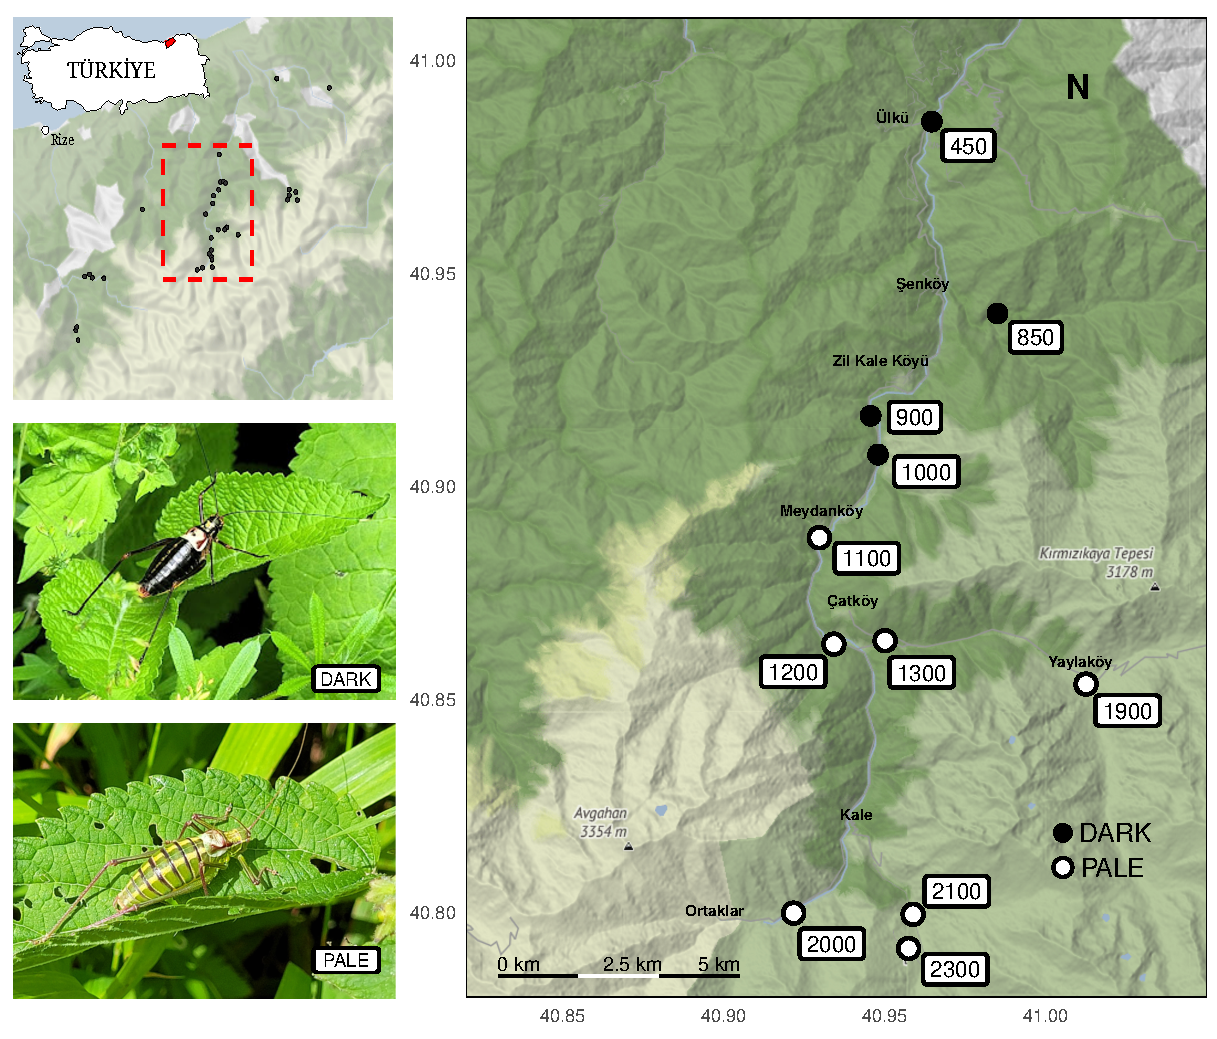
\includegraphics[width=1.8\columnwidth]{Figure_1.pdf}
\caption{Sampling locations of \textit{I. rizeensis} in the Fırtına Valley, Türkiye. Map showing the 11 collection sites along an altitudinal gradient within the Fırtına Valley. Village names and elevation values (in meters) are indicated. Sampling locations are categorized based on the two major color morphs of \textit{I. rizeensis} dark and pale.}
\label{Figure 1}
\end{figure}

\clearpage
\newpage
\begin{figure}[h]
\centering
\includegraphics[width=1.8\columnwidth]{Figure_2.pdf}
\caption{Genetic structure and differentiation of \textit{I. rizeensis} along an alitudinal gradient in the Fırtına Valley. \textbf{(A)} Principal Component Analysis (PCA) of genetic variation, showing genetic structuring between lower-altitude (dark-colored) and higher-altitude (pale-colored) individuals along PC1. \textbf{(B)} Admixture proportions for $K=3$, illustrating distinct genetic ancestries at low (black) and high (green) altitudes, with mid-altitude populations exhibiting mixed ancestry. \textbf{(C)} Isolation-by-distance (IBD) pattern revealed by Mantel tests, showing significant patterns of genetic differentiation along the altitudinal gradient as measured by $F_{ST}$}
\label{Figure 2}
\end{figure}

\clearpage
\newpage
\begin{figure}[h!]
\centering
\includegraphics[width=0.8\columnwidth]{Figure_3.pdf}
\captionsetup[table]{labelsep=space, 
        justification=raggedright, singlelinecheck=off}
    \caption{Nucleotide diversity (A) and genetic differentiation (B) for adaptive and neutral loci in \textit{I. rizeensis} along an alitudinal gradient in the Fırtına Valley}
\label{Figure 3}
\end{figure}
\newpage
\begin{figure}[h!]
\centering
\includegraphics[width=0.8\columnwidth]{Figure_4.pdf}
\caption{Altitudinal variation in allele frequencies for the 102 SNPs significantly associated with elevation in \textit{I. rizeensis}, showing two distinct trends where the minor allele frequency either increases or decreases with altitude.}
\label{Figure 4}
\end{figure}

\begin{figure*}[b!]
\centering
\includegraphics[width=1.8\columnwidth]{Figure_5.pdf}
\caption{Genetic differentiation between dark and pale color morphs of \textit{I. rizeensis} based on Discriminant Analysis of Principal Components (DAPC). (A) DAPC density plot along Discriminant Function 1 (DF1), showing clear separation between the morphs. (B) SNP loadings on DF1 identifying three major-effect loci contributing to morph differentiation. (C) Genotypic states at the three major loci along the altitudinal gradient. HMJ = Homozygote Major; HT = Heterozygote; HMN = Homozygote Minor}
\label{Figure 5}
\end{figure*}

\end{document}